% Chapter 4

\chapter{后端设计}

\section{概述}

本系统的后端整体上是基于Spring Boot框架开发起来的,代码用Java编写。图\ref{fig:package}是以包为单位绘制的,一个简要的后端代码结构关系图。

\begin{figure}[!htb]
	\centering
	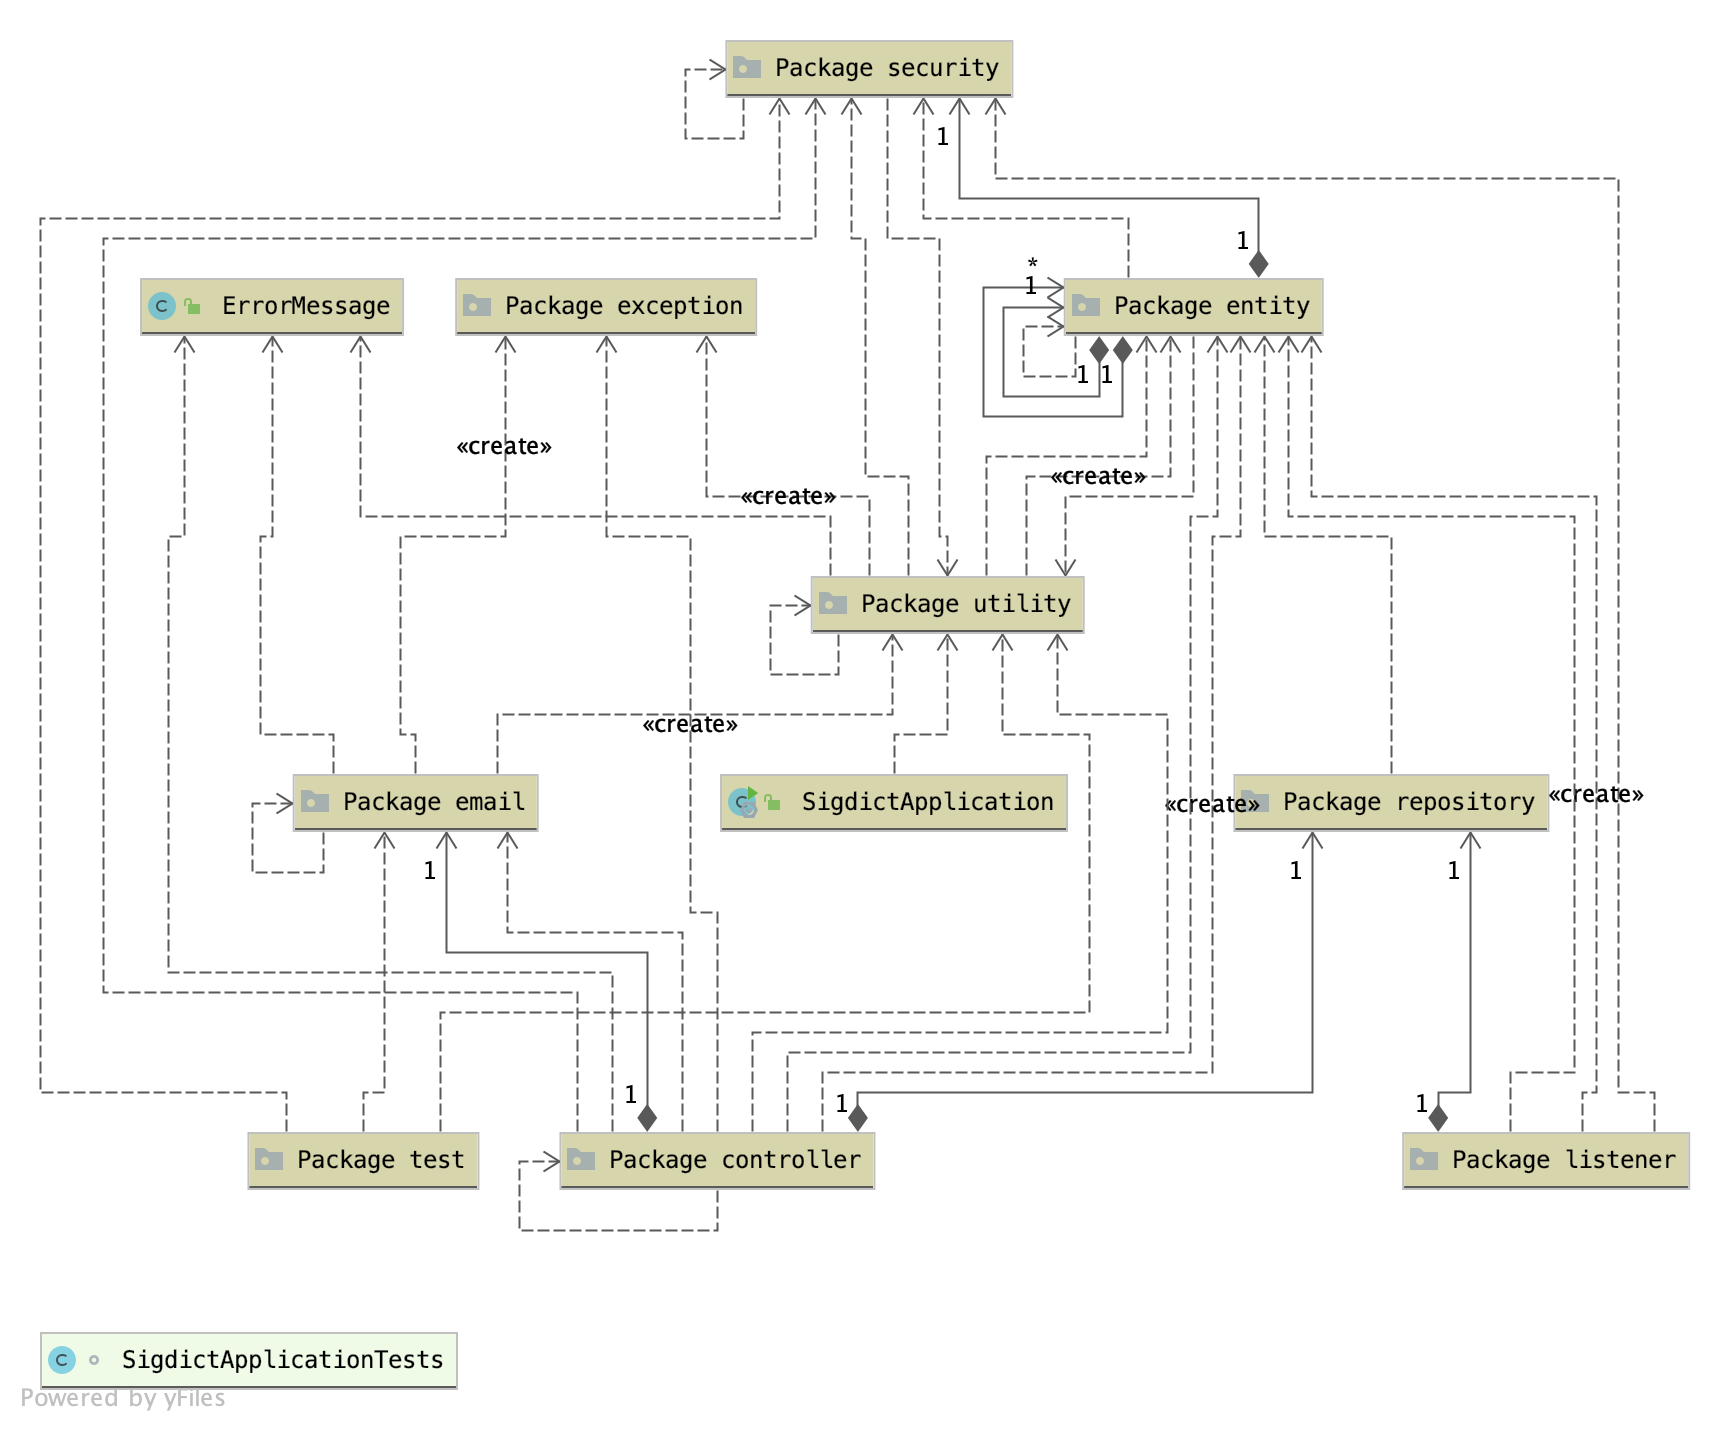
\includegraphics[width=0.8\textwidth]
	{figures/package.png}\\
	\caption{后端Java代码的关系图}
	\label{fig:package}
\end{figure}

\begin{itemize}

	\item \textbf{Package email}
	
	包含了有关发送电子邮件的代码,详见小节\ref{sec:emailP}。
	
	\item \textbf{Package controller}
	
	包含了所有Controller类,详见小节\ref{sec:controllerP}。
	
	\item \textbf{Package exception}
	
	包含了所有我们自己定义的Exception类型。
	
	\item \textbf{Package listener}
	
	定义了一个用于在Spring Boot框架基本完成启动时触发的监听器。这个监听器将负责为项目进行一些初始化工作,例如生成主密钥(详见小节\ref{sec:keyS})。
	
	\item \textbf{Package test}
	
	包含了一些对于部分代码简单的单元测试。
	
	\item \textbf{Package entity}
	
	作为MVC模型中的Model,与Package repository一起在Hibernate的帮助下完成了用操作对象的方式进行数据库操作。
	
	\item \textbf{Package repository}
	
	包含了所有的repository类,与Package entity一起在Hibernate的帮助下完成了用操作对象的方式进行数据库操作。
	
	\item \textbf{Package security}
	
	包含了所有安全相关的函数。
	
	\item \textbf{Package utility}
	
	包含了所有辅助类的类、方法。

\end{itemize}

\section{发送电子邮件服务}\label{sec:emailP}

我们将通过JavaMail库的帮助与一个SMTP服务器建立联系,并最终将邮件推送到用户的设备上,相关代码位于包email中。

因为Google提供小规模免费的SMTP服务,我们这里就以Google的SMTP服务为例。为了成功的发送电子邮件,我们首先需要配置相应的SMTP服务器地址和端口,下方代码片段示例的4-5行完成了这项工作。同时往往提供这类服务的服务器需要使用者登录,因此在第10行完成了用用户名、密码登录验证的操作。

\begin{minted}
[
	frame=lines,
	framesep=2mm,
	baselinestretch=1.2,
	bgcolor=lightgray,
	fontsize=\footnotesize,
	linenos
]{java}

Properties props = new Properties();
props.put("mail.smtp.auth", "true");
props.put("mail.smtp.starttls.enable", "true");
props.put("mail.smtp.host", "mail.smtp.host");
props.put("mail.smtp.port", "587");

Session session = Session.getInstance(props,
        new javax.mail.Authenticator() {
                protected PasswordAuthentication getPasswordAuthentication() {
                        return new PasswordAuthentication(username, password);
                }
        }
);

\end{minted}

这之后只需要如下代码片段所示,将邮件的收件人地址、主体、正文等信息设置妥当后,就可以执行发送的命令,送出这份电子邮件。我们所选择的SMTP服务器在收到这封电子邮件后,将会尝试将它推送给接收用户所属的SMTP服务器。在推送成功后,接收用户便可以从所属的SMTP服务器中拉取、查看这封电子邮件。

\begin{minted}
[
	frame=lines,
	framesep=2mm,
	baselinestretch=1.2,
	bgcolor=lightgray,
	fontsize=\footnotesize,
	linenos
]{java}

Message message = new MimeMessage(session);
message.setFrom(new InternetAddress(fromEmail));
message.setRecipients(Message.RecipientType.TO, InternetAddress.parse(toEmail));
message.setSubject(subject);
message.setText(content);
Transport.send(message);

\end{minted}

发送电子邮件因为涉及网络IO交互,所以相比于其他操作会产生巨大的延迟。为了提高响应速度,让用户拥有更好的使用体验,我们利用Spring Boot的@Async关键词对本模块做了一层封装修饰。让发送方式从同步阻塞变成异步非阻塞,增加效率,显著减少了用户需要等待的时间。但这样做有利有弊,缺点是即使服务器端发生错误(如500服务器内部错误),导致电子邮件发送失败,用户也无法得到相应的错误提示,用户会错以为我们已经正确的发送了电子邮件。

\section{用户Session的维护}

用户需要登录后才能进行上传文件、下载文件、查看文件数字签名等操作。因为我们必须在用户登录后在服务器端记录一些信息,用于维持用户的登录状态,在这里我们采用了生成Session的方式维持该状态。

具体而言,用户在成功的登录之后,服务器端会随机的生成一个长度为16字节的二进制数据,并将其转化为base64编码\cite{base64}作为用户的Session。这个Session数据首先会被存储在服务器端数据库中,然后会被通过Cookie\cite{cookie}的方式返还给用户。之后用户每次访问我们网站的时候浏览器都会把这个Cookie发送给服务器端,我们会将之与数据库中的信息进行对比,判断用户所处的状态,并给出不同的响应结果。

关于Session的安全分析详见小节\ref{sec:sessionS}。

\section{Controller}\label{sec:controllerP}

Controller作为一个MVC框架的组成部分在网站的整体响应过程中起着至关重要的作用。表\ref{tab:controller}简要列举了我们设计的所有Controller类。

\begin{table}[ht]
\centering
\begin{tabular}{>{\bfseries}lp{9cm}}
\toprule
SessionController & 
一个抽象类,包含了一些用于验证、管理Session的方法,其他所有需要处理Session的Controller都将继承该类。\\
\midrule
EmailController & 
继承自SessionController,负责处理与电子邮件相关的请求。\\
\midrule
IndexController & 
继承自SessionController,负责处理与欢迎界面相关的请求。\\
\midrule
LoginController &
继承自SessionController,负责处理与登录相关的请求。\\
\midrule
LogoutController &
继承自SessionController,负责处理与登出相关的请求。\\
\midrule
MessageController &
继承自SessionController,负责处理与信息界面相关的请求。\\
\midrule
FileController &
继承自SessionController,负责处理与文件相关的请求,包括上传文件、下载文件、删除文件等。\\
\midrule
KeyController &
继承自SessionController,负责处理与密钥相关的请求。\\
\midrule
PasswordController &
继承自SessionController,负责处理与密码的请求,包括更改密码,忘记密码、重置密码等。\\
\midrule
MainController &
继承自SessionController,负责处理与主页面相关的请求。\\
\midrule
RegisterController &
继承自SessionController,负责处理与注册页面相关的请求。\\
\midrule
SigdictErrorController &
负责处理与错误页面相关的请求。\\
\bottomrule
\end{tabular}
\caption{Controller类}
\label{tab:controller}
\end{table}

我们以处理访问主界面请求的MainController为例,Spring Boot框架使用(如下所示代码第1行的)@RequestMapping装饰器将用户的请求映射到某个具体的响应方法中。通过调整响应的参数,我们可以指定映射URL的样式(/main.html),同时可以指定映射的方法类型(GET、POST、DELETE等)。

通常而言,我们在处理请求时需要做的第一件事是验证用户的状态,如下图代码第5行所示。validateSession()方法从抽象类SessionController中继承而来,它会从用户的请求附带的cookies中提取出session(如存在),然后与我们数据库中的数据进行对比,从而确认用户的身份、以及其所处的状态。

如下图代码第6-11行所示,如果validateSession()返回的用户为空,则代表用户并没有登录,处于非法状态,在这个时候我们会把请求重定向到登录界面,要求用户输入用户名、密码登录,并附带上响应的错误提示信息。

如下图代码第12-14行所示,如果用户登录状态正确,我们会交给Thymeleaf渲染出正确的主界面并返回会给用户,同时用户的部分个人信息也会显示出来。

\begin{minted}
[
	frame=lines,
	framesep=2mm,
	baselinestretch=1.2,
	bgcolor=lightgray,
	fontsize=\footnotesize,
	linenos
]{java}

@RequestMapping(value = "/main.html", method = RequestMethod.GET)
public String getMainPage(Model model,
                                        HttpServletRequest request,
                                        RedirectAttributes redirectAttributes) {
        User user = validateSession(request);
        if (user == null) { // haven't signed in
                PassMessage.addRedirectAttributesErrorMessage(
                        redirectAttributes, 
                        ErrorMessage.SIGH_IN_FIRST);
                return "redirect:/login.html";
        }
        PassMessage.addUserMessage(model, user);
        PassMessage.addModelMainPageFiles(model, user);
        return "main";
}

\end{minted}

\section{数据库设计}

数据库是可持久化存储数据的重要一环,为项目的稳定性提供了重要的保障。图\ref{fig:db}是我们设计的后端数据库存储方案。我们总共设计了包括USER,UPLOADED\_FILE等在内的6个表格,它们之间通过一定的外键约束在一起。

\begin{figure}[!htb]
	\centering
	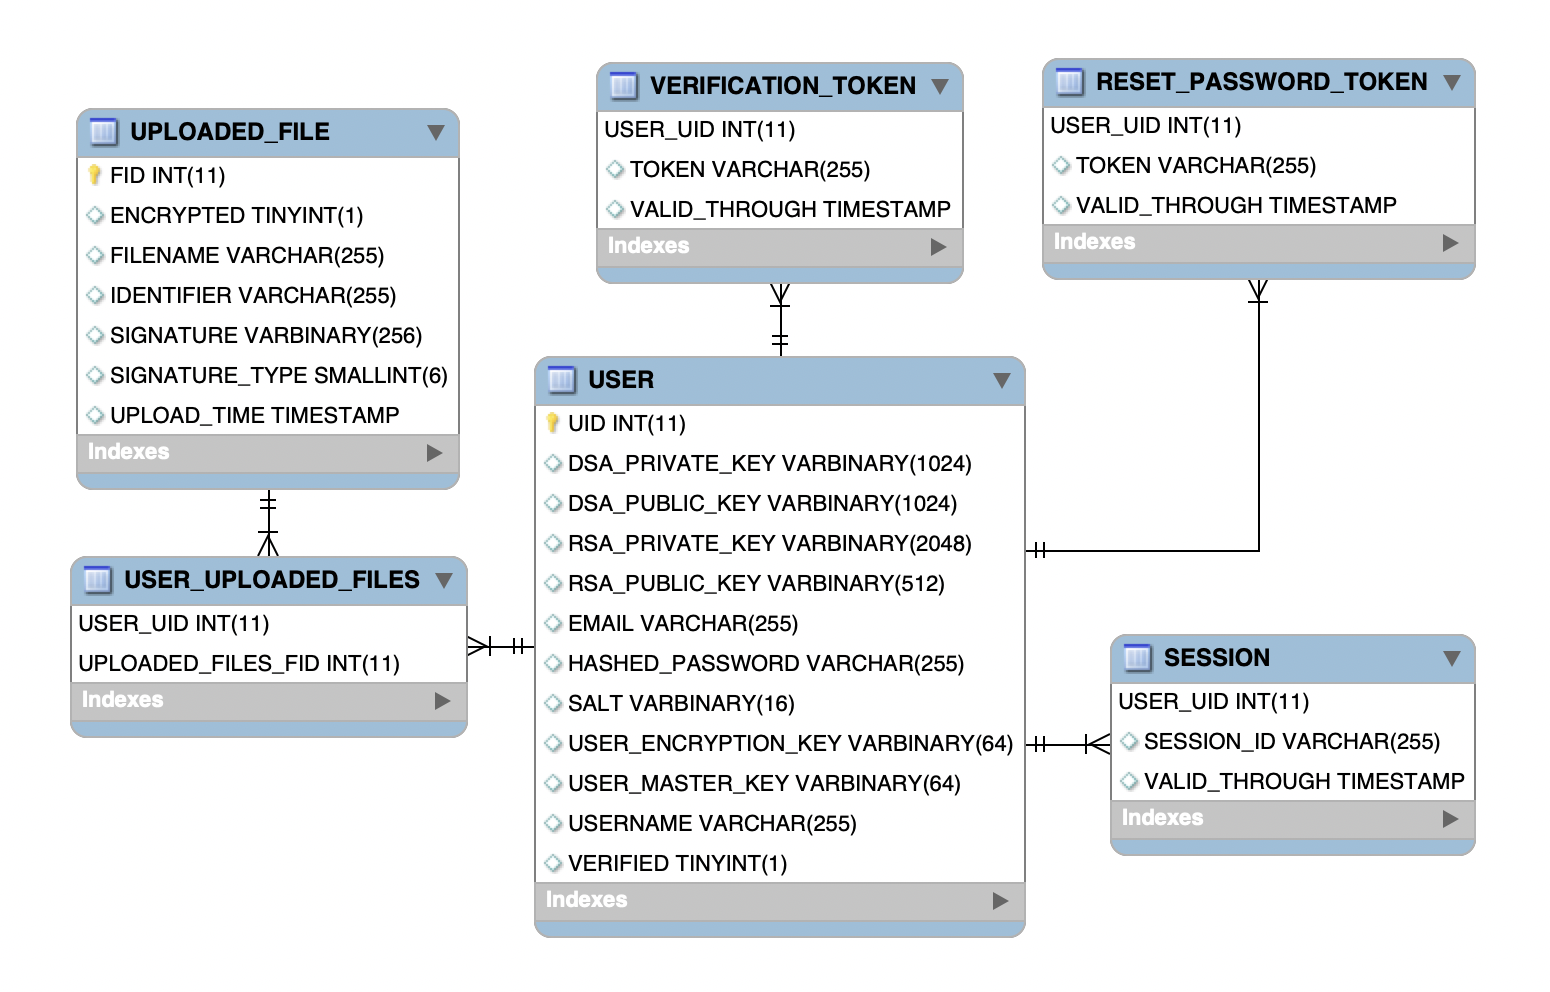
\includegraphics[width=0.8\textwidth]
	{figures/db.png}\\
	\caption{数据库表关系图}
	\label{fig:db}
\end{figure}

\begin{itemize}
	\item \textbf{USER}
	
	USER表格使我们存储系统中最为核心的一张数据表。在其中存储了包含用户ID,用户名,邮箱,哈希过后的密码(见小节\ref{sec:hashpassword})以及多个密钥等关键信息。
	
	\item \textbf{UPLOADED\_FILE}
	
	UPLOADED\_FILE表格存储着用户所上传文件的相关信息。其中包括文件ID,是否加密,文件名,上传时间,签名类型,数字签名,文件标识符(见小节\ref{sec:fileV})等信息。
	
	\item \textbf{USER\_UPLOADED\_FILE}
	
	USER\_UPLOADED\_FILE表格作为桥梁,记录着用户与文件之间的对应关系,这是潜在的多对多数据关系,所以我们单独用拆开用一个表格记录该数据。USER\_UPLOADED\_FILE表格通过两个外键约束与USER表格和UPLOADED\_FILE表格联系在一起。
	
	\item \textbf{SESSION}
	
	SESSION表格用于记录维持用户登录状态所需要的相关信息,包括Session ID,用户ID和有效期限等。
	
	\item \textbf{RESET\_PASSWORD\_TOKEN}
	
	RESET\_PASSWORD\_TOKEN表格主要记录向用户发送重置密码链接所需要的相关信息,包含Token ID,用户ID和有效期限等。
	
	\item \textbf{VERIFICATION\_TOKEN}
	
	VERIFICATION\_TOKEN表格主要记录向用户发送验证邮箱链接所需要的相关信息,包含Token ID,用户ID和有效期限等。
	
\end{itemize}

值得注意的是SESSION表,RESET\_PASSWORD\_TOKEN表和VERIFICATION\_TOKEN表其实,与USER表格实际上是一对一关系的,即一个用户只能拥有一个Session,一个用户只能拥有一个重置密码链接,一个用户只能拥有一个验证邮箱链接。

也就是说这三张表格其实完全可以合并入USER表格中,但我们没有这样做。原因是我们希望能尽可能的优化数据库存储空间的利用率。因为在同一时刻必定只有总体用户中的一小部分才会真的拥有上述三种信息,而如果将它们合并进入USER表格中,势必会产生大量的无效数据(以NULL或其他特殊数值表示的非法标记)。这将会白白占用大量的数据库存储空间。

下面以Session为例,简要展示一下如何通过Hibernate以操作对象的方式进行数据库读写。下图所示代码是entity/Session.java中的部分代码示例。

可以看到,在第1行,我们用@Entity装饰器让Hibernate接管这个类。随后在第4-7行定义了一些需要的成员变量,这些成员变量也将被Hibernate映射到底层数据库表格中的一列。第三行@Id装饰器表明uid是主键。同时第8-11行我们使用了@OneToOne和@MapsId装饰器将Session与User通过外键的形式连接、映射在了一起。

\begin{minted}
[
	frame=lines,
	framesep=2mm,
	baselinestretch=1.2,
	bgcolor=lightgray,
	fontsize=\footnotesize,
	linenos
]{java}

@Entity // This tells Hibernate to make a table out of this class
public class Session {
        @Id
        private Integer uid;
        private String sessionId;
        @Basic
        private Timestamp validThrough;
        @OneToOne
        @MapsId // @MapsId tells Hibernate to use the id column of 
        // this entity as both primary key and foreign key.
        private User user;
        // other methods are omitted, including getters and setters
}

\end{minted}

下面所示代码是repository/SessionRepository.java中的部分片段。

在Controller中,我们将通过操作SessionRepository来获取某个具体的Session对象,这里我们定义了findBySessionId方法,使得我们可以通过sessionID查找相应的Session对象。而Controller中的repository对象则用@Autowired装饰器修饰,Spring Boot框架将会在运行时自动绑定一个repository添加进去。

\begin{minted}
[
	frame=lines,
	framesep=2mm,
	baselinestretch=1.2,
	bgcolor=lightgray,
	fontsize=\footnotesize,
	linenos
]{java}

public interface SessionRepository extends CrudRepository<Session, Integer> {
        Session findBySessionId(String sessionId);
}

\end{minted}

